% This section presents additional details and experimental results omitted from
% the main body of the paper. 
In addition to the \texttt{mg\_scale} dataset presented in
Section~\ref{s:experiments}, we also benchmarked on three other data sets
described in Table~\ref{tab:libsvm-datasets}.
\begin{table}[ht]
  \centering
  \caption{Datasets used in the experiments \citep{libsvm}.}
  \label{tab:libsvm-datasets}
  \begin{tabular}[t]{lcccc}
    \toprule
        & \texttt{mg\_scale} & \texttt{bodyfat\_scale} & \texttt{mpg\_scale} & \texttt{housing\_scale} \\
    \midrule
    $n$ & 1385               & 252                     & 392                 & 506                     \\
    $d$ & 6                  & 14                      & 7                   & 13                      \\
    \bottomrule
  \end{tabular}
\end{table}

The A-optimality values obtained are illustrated in Figure~\ref{f:obj-grid}.
The general trend observed in Section~\ref{s:experiments} of our method
(without SDP) outperforming independent sampling methods (uniform and
predictive length) and our method (with SDP) matching the performance of the
greedy bottom up method continues to hold across the additional datasets considered.

\begin{figure}[htpb]
  \centering
  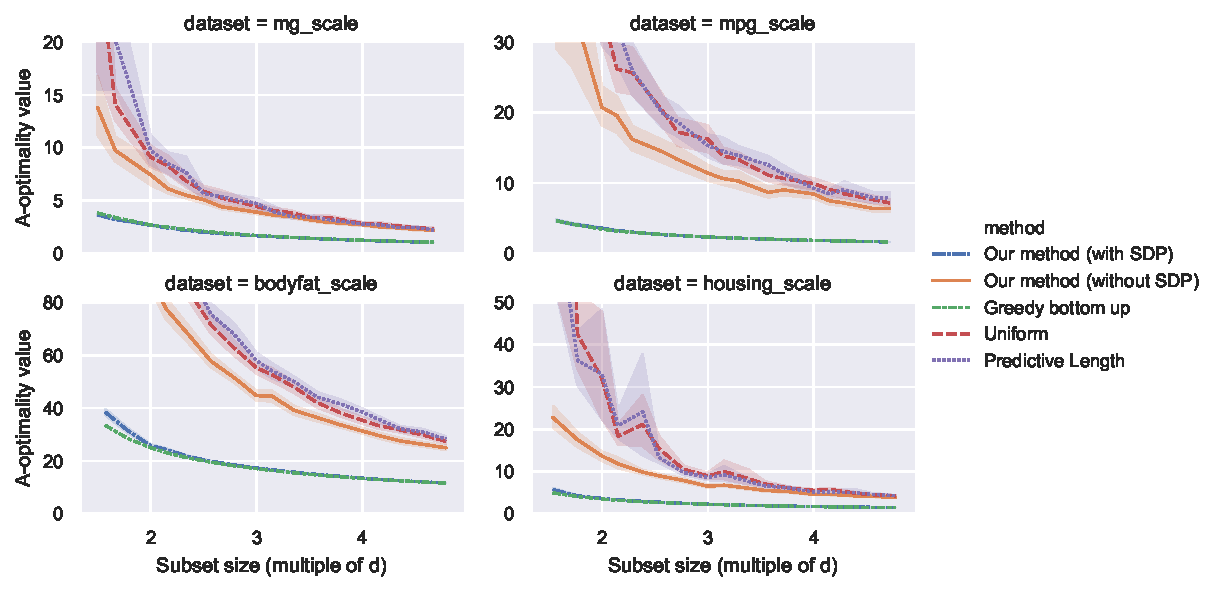
\includegraphics[width=\textwidth]{design/bayesian_figures/obj_grid.pdf}
  \caption{A-optimality values achieved by the methods compared. In all cases
    considered, we found our method (without SDP) to be superior to independent
    sampling methods like uniform and predictive length sampling. After paying the price
    to solve an SDP, our method (with SDP) is able to consistently match the performance
    of a greedy method which has been noted
    \citep{chamon2017approximate} to work well empirically.}
  \label{f:obj-grid}
\end{figure}

The relative ranking and overall order of magnitude differences
between runtimes (Figure~\ref{f:runtimes}) are also similar across the various
datasets. An exception to the rule is on $\texttt{mg\_scale}$, where we see
that our method (without SDP) costs more than the greedy method
(whereas everywhere else it costs~less).

\begin{figure}[htpb]
  \centering
  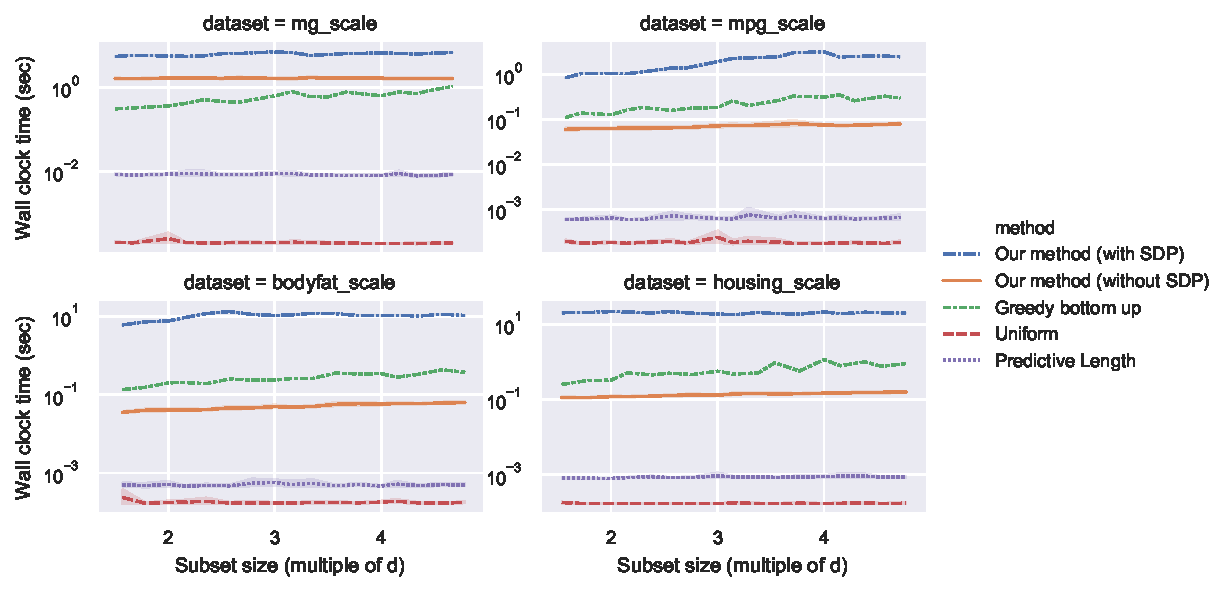
\includegraphics[width=\textwidth]{design/bayesian_figures/runtime_grid.pdf}
  \caption{Runtimes of the methods compared. Our method (without SDP) is
    within an order of magnitude of greedy bottom up and faster in 3 out of
    4 cases. The gap between our method with and without SDP is
    attributable to the SDP solver, making investigation of more efficient
    solvers and approximate solutions an interesting direction for future
    work.
  }
  \label{f:runtimes}
\end{figure}

The claim that $f_{\A}(\frac{k}{n} \Sigmab_\X)$ is an appropriate
quantity to summarize the contribution of problem-dependent factors
on the performance of Bayesian A-optimal designs is further evidenced in Figure~\ref{f:ratios}.
Here, we see that after normalizing the A-optimality values by this
quantity, the remaining quantities are all on the same scale and close to $1$.

\begin{figure}[htpb]
  \centering
  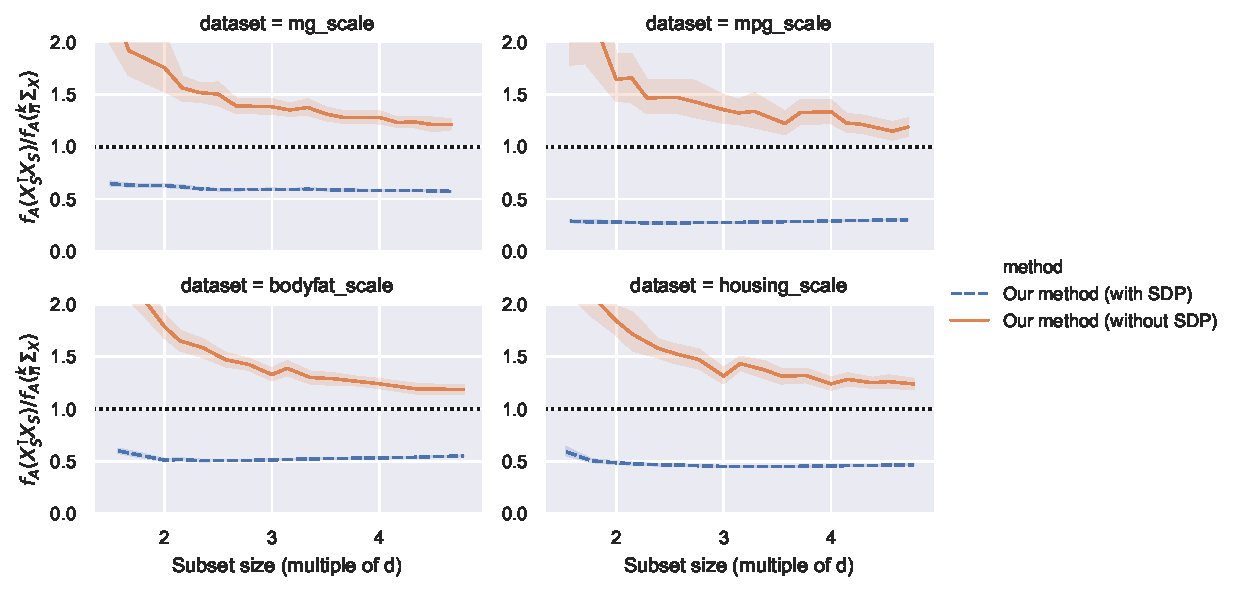
\includegraphics[width=\textwidth]{design/bayesian_figures/ratios_grid.pdf}
  \caption{The ratio controlled by Lemma~\ref{l:guarantees}. This ratio converges
    to $1$ as $k \to n$ and is close to $1$ across all
    real world datasets,
    suggesting that $f_{\A}(\frac{k}{n} \Sigmab_\X)$
    is an appropriate problem-dependent scale for Bayesian A-optimal
    experimental design.
  }
  \label{f:ratios}
\end{figure}

% The choice of $\lambda=43$ is motivated by keeping 95\% of the spectral
% mass. Figure~\ref{fig:scree} shows a scree plot for \texttt{mpg\_scale}
% after applying a polynomial kernel, where we see that the majority
% of the spectral mass is contained in the top few eigenvalues.

% \begin{figure}[htbp]
%     \centering
%     % \hspace{-0.55cm}
%     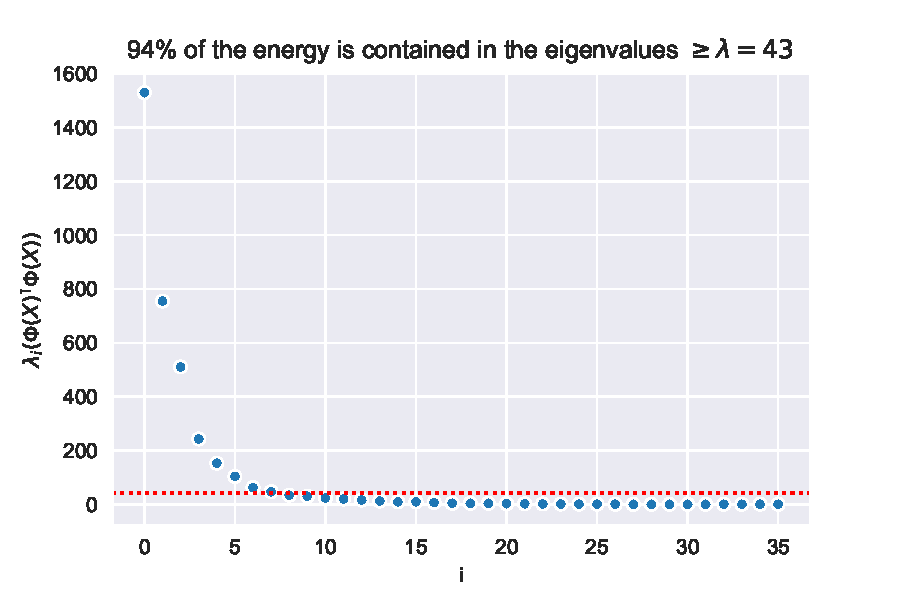
\includegraphics[width=0.5\textwidth]{Figures/screeplot.pdf}
%     \caption{
%         To determine the amount of regularization $\lambda$, a scree
%         plot of the eigenvalues of the polynomially expanded
%         covariance matrix $\Phi(X)^\top \Phi(X)$.
%     }
%     \label{fig:scree}
% \end{figure}

